\documentclass[dvipdfmx]{beamer}
\usepackage{tutorial}
\title{計算機実験 --- 数値計算の基礎}
\author{藤堂眞治}
\date{2015-09-24}

\begin{document}

\begin{frame}
  \titlepage
  \tableofcontents
\end{frame}

\section{講義・実習の概要}

\begin{frame}[t]{講義・実習の目的}
  \begin{itemize}
    %\setlength{\itemsep}{1em}
  \item 理論・実験を問わず、学部〜大学院〜で必要となる現代的かつ普遍的な計算機の素養を身につける
    \begin{itemize}
    \item UNIX環境に慣れる(シェル、ファイル操作、エディタ)
    \item ネットワークの活用 (リモートログイン、バージョン管理、共同作業)
    \item プログラムの作成(C言語、コンパイラ、プログラム実行)
    \item 基本的な数値計算アルゴリズム・数値計算の常識を学ぶ
    \item 科学技術文書作成に慣れる(\LaTeX, グラフ作成)
    \item Mathematica, Pythonなどのツールの利用
    \end{itemize}
  \item ツールとしてないものは自分で作る (物理の伝統)
  \item すでにあるものは積極的に再利用する (車輪の再発明をしない)
  \item 数値計算においても再現性は重要
  \end{itemize}
\end{frame}

\begin{frame}[t]{講義内容}
  \begin{enumerate}
    \setlength{\itemsep}{1em}
  \item UNIXの操作、ネットワーク
  \item プログラミング: C言語、数値計算ライブラリの利用
  \item ツール: エディタ、コンパイラ、\LaTeX、Gnuplot、バージョン管理システム、Mathematica、Python
  \item 数値計算アルゴリズム: 数値微分、ニュートン法、数値積分、常微分方程式、連立一次方程式、対角化、特異値分解、最小二乗法、最適化手法、モンテカルロ法
  \item その他の話題: スーパーコンピュータ、並列化、シミュレーションパッケージの利用
  \end{enumerate}
\end{frame}

\begin{frame}[t]{講義資料}
  \begin{itemize}
    \setlength{\itemsep}{1em}
  \item 「計算機実験」ハンドブック (配布済)
    \begin{itemize}
    \item UNIX入門
    \item C言語入門
    \item \LaTeX 入門
    \end{itemize}
  \item 講義資料、実習資料、追加資料、参考書
    \begin{itemize}
    \item ITC-LMSで配布・提示 \url{https://itc-lms.ecc.u-tokyo.ac.jp/lms/course/view.php?id=74564}
    \end{itemize}
  \end{itemize}
\end{frame}

\begin{frame}[t,fragile]{実習を始めるために最低限必要な知識}
  \begin{itemize}
    \setlength{\itemsep}{1em}
  \item ハンドブック 2章 UNIX入門
    \begin{itemize}
    \item 2.1 UNIXのコマンド (2.1.1)
    \item 2.2 リモートログインとファイル転送
    \item 2.3 Emacsを使う (2.3.2) (viを使ってもよい)
    \item 2.4 Gnuplotを使う
    \end{itemize}
  \item ハンドブック 3章 C言語入門
    \begin{itemize}
    \item 3.1 C言語の基礎知識 (3.1.1, 3.1.2, 3.1.3)
    \item 3.2 制御文 (3.2.1, 3.2.2)
    \item 3.6 関数 (3.6.2)
    \end{itemize}
  \item ハンドブック 4章 \LaTeX 入門
    \begin{itemize}
    \item 4.1 \LaTeX の実行
    \end{itemize}
  \end{itemize}    
\end{frame}

\begin{frame}[t]{質問がある場合には、、、}
  \begin{enumerate}
    %\setlength{\itemsep}{1em}
  \item ITC-LMS の掲示板を見る
  \item ハンドブック、講義資料を確認
  \item ネットで検索
  \item ワークグループのメンバーに相談する
  \item 計算機実験担当者(藤堂、諏訪、鈴木、足立、安藤) \href{mailto:computer@exa.phys.s.u-tokyo.ac.jp}{computer@exa.phys.s.u-tokyo.ac.jp} に相談
  \end{enumerate}
  質問するときに注意すべきこと
  \begin{itemize}
  \item (メールの)標題をきちんとつける、きちんと名乗る
  \item 実行環境を明示する
  \item 問題を再現する手順を明記する
  \item 関連するファイル(Cや \LaTeX のソースコード等)を添付する
  \item エラーメッセージを添付する
  \end{itemize}
\end{frame}

\begin{frame}[t,fragile]{実習環境}
  \begin{itemize}
    \setlength{\itemsep}{1em}
  \item 情報基盤センター大演習室 (iMac端末)
    \begin{itemize}
    \item Cプログラミング、\LaTeX、Gnuplot、Mathematicaなどに利用
    \end{itemize}
  \item 計算機端末室
    \begin{itemize}
    \item 理学部1号館317室 (iMac 20台)
    \item 月曜10:00-金曜19:00に利用可
    \end{itemize}
  \item MateriApps LIVE!
    \begin{itemize}
    \item Mac, Windows PC 上で動作する仮想UNIX環境
    \item インストール方法はUSB内の\href{https://github.com/cmsi/MateriAppsLive/wiki/MateriAppsLive-ltx}{README.html}を参照
    \end{itemize}
  \end{itemize}
\end{frame}

\section{数値誤差}

\begin{frame}[t,fragile]{数値誤差の原因}
  \begin{itemize}
    \setlength{\itemsep}{1em}
  \item 丸め誤差: 無理数や10進数を有限のビットの2進数で表現することによる誤差
    (例: 0.1 が 0.0999999999998 になる)
  \item 打ち切り誤差: テイラー展開による近似を有限項で打ち切ることによる誤差
    (例: 数値微分)
  \item 桁落ち: 非常に近い数の引き算により生じる
  \item 情報落ち: 非常に大きな数に小さな数を足し込む場合に生じる
    (例: 数値積分や常微分方程式の初期値問題で刻み幅を小さくしすぎると生じる)
  \item オーバーフロー(桁あふれ): 表現できる値を超えてしまう
  \end{itemize}
\end{frame}

\begin{frame}[t,fragile]{桁落ち}
  \begin{itemize}
    \setlength{\itemsep}{1em}
  \item 2次方程式 $ax^2+bx+c=0$の解の公式
    \[
    x_{\pm} = \frac{-b \pm \sqrt{b^2-4ac}}{2a}
    \]
    $b^2 \gg |ac|$の時、桁落ちが生じる
  \item 例) $2.718282x^2 - 684.4566x+0.3161592=0$ の解を7桁の精度で計算してみる(伊理・藤野1985)
    \begin{align*}
      \sqrt{D} &= \sqrt{(684.4566)^2 - 4 \times 2.718282 \times 0.3161592} = 684.4541 \\
      x_+ &= \frac{684.4566+684.4541}{2 \times 2.718282} = \frac{1368.911}{5.436564} = 251.7970 \\
      x_- &= \frac{684.4566-684.4541}{2 \times 2.718282} = \frac{0.0025}{5.436564} = 0.00045\underline{98493}
    \end{align*}
  \end{itemize}
\end{frame}

\begin{frame}[t,fragile]{桁落ちを防ぐ方法}
  \begin{itemize}
    \setlength{\itemsep}{1em}
  \item $b$の符号に応じて、一方を求める(この例では$x_+$)
  \item 他方は解と係数の関係を使って求める
    \[
    x_- = \frac{c/a}{x_+} = \frac{0.3161592 / 2.718282}{251.7970} = 0.000461913\underline{8}
    \]
  \item 回避できない例: 重解に近い場合 $2.718282x^2 - 1.854089x + 0.3161592=0$
    \begin{align*}
      \sqrt{D} &= \sqrt{(1.854089)^2 - 4 \times 2.718282 \times 0.3161592} \\ &= 0.002\underline{64575} \\
      x_\pm &= 1.854089 \pm 0.002\underline{64575} = 1.856\underline{737}, 1.851\underline{445}
    \end{align*}
  \end{itemize}
\end{frame}

\begin{frame}[t,fragile]{数値微分}
  \begin{itemize}
    \setlength{\itemsep}{1em}
  \item 関数のテイラー展開
    \[
    f(x+h) = f(x) + h f'(x) + h^2 f''(x)/2 + h^3 f'''(x)/6 + \cdots
    \]
  \item 数値微分の最低次近似
    \[
    f_1(x,h) \equiv \frac{f(x+h)-f(x)}{h} = f'(x) + h f''(x)/2 + O(h^2)
    \]
  \item より高次の近似
    \[
    f_2(x,h) \equiv \frac{f(x+h)-f(x-h)}{2h} = f'(x) + h^2 f'''(x)/6 + O(h^3)
    \]
  \item 刻み$h$を小さくすると打ち切り誤差は減少するが、小さすぎると今度は桁落ちが大きくなる
  \end{itemize}
\end{frame}

\begin{frame}[t,fragile]{刻み幅を変えた計算}
  \begin{itemize}
    \setlength{\itemsep}{1em}
  \item 刻み幅を変えて何度か計算を行い、収束の様子をみる
  \item グラフ化して目で見てみる
  \item 理論式と比較
    \begin{itemize}
    \item 計算式の正しさの確認
    \item 近似の改良 (収束の加速・補外)
    \end{itemize}
  \item 桁落ち・情報落ちの影響の有無
  \end{itemize}
\end{frame}

\section{ニュートン法}

\begin{frame}[t,fragile]{ニュートン法}
  \begin{itemize}
    \setlength{\itemsep}{1em}
  \item 反復法により方程式$f(x)=0$の解を求める
  \item 真の解を$x_0$、適当な解の候補を$x'=x_0+\epsilon$とすると
    \[
    0 = f(x_0) = f(x_0+\epsilon-\epsilon) = f(x') - \epsilon f'(x') + O(\epsilon^2)
    \]
  \item 次の解の候補 (反復法、逐次近似法)
    \[
    x'' = x'-\epsilon \approx x' - \frac{f(x')}{f'(x')}
    \]
  \item 複素変数の複素関数や多変数の場合にも自然に拡張可
  \end{itemize}
\end{frame}

\begin{frame}[t,fragile]{ニュートン法の収束}
  \begin{itemize}
    \setlength{\itemsep}{1em}
  \item $x'$が$x_0$に十分近い時
    \begin{align*}
      f(x') &\approx (x'-x_0) f'(x_0) + \frac{(x' - x_0)^2}{2} f''(x_0) \\
      f'(x') &\approx f'(x_0) + (x' - x_0) f''(x_0)
    \end{align*}
  \item ニュートン法で一回反復すると
    \begin{align*}
      x'' =  x' - \frac{f(x')}{f'(x')} &\approx x' - (x'-x_0)(1-\frac{(x'-x_0)}{2}\frac{f''}{f'}) \\
      (x''-x_0) &\approx \frac{f''}{f'} (x' - x_0)^2
    \end{align*}
    \item 一回の反復で誤差が2乗で減る(正しい桁数が倍に増える) ⇒ 二次収束
  \end{itemize}
\end{frame}

\section{代数方程式の解法}

\begin{frame}[t,fragile]{代数方程式}
  \begin{itemize}
    \setlength{\itemsep}{1em}
  \item 実係数の$n$次方程式
    \[
    P(z) = z^n + a_1 z^{n-1} + \cdots + a_n = 0
    \]
  \item ニュートン法 + 減次 (次数低下法)
    \begin{itemize}
    \item ニュートン法により一つの解($\alpha$)を求める
    \item $g(x) = f(x) / (x-\alpha)$の解として、他の解を逐次求めていく
    \item 毎回誤差がたまっていくため、解はくずれていく
    \end{itemize}
  \end{itemize}
\end{frame}


\begin{frame}[t,fragile]{Durand-Kerner-Aberth法 (Wierstrass法)}
  \begin{itemize}
    \setlength{\itemsep}{1em}
  \item 真の解を$\alpha_1,\alpha_2,\cdots,\alpha_n$とすると
    \[
    P(z) = (z-\alpha_1) (z-\alpha_2) \cdots (z-\alpha_n)
    \]
  \item $\alpha_1,\alpha_2,\cdots,\alpha_n$に現在の近似解$z^{(\nu)}_1,z^{(\nu)}_2,\cdots,z^{(\nu)}_n$を代入し、$z=z^{(\nu)}_k$における微分の値を評価
    \[
    P'(z^{(\nu)}_k) \approx \prod_{j \ne k} (z^{(\nu)}_k - z^{(\nu)}_j)
    \]
  \item ニュートン法による反復
    \[
    z^{(\nu+1)}_k = z^{(\nu)}_k - \frac{P(z^{(\nu)}_k)}{\prod_{j \ne k} (z^{(\nu)}_k - z^{(\nu)}_j)}
    \]
  \end{itemize}
\end{frame}

\begin{frame}[t,fragile]{初期値の選び方}
  \begin{itemize}
    \setlength{\itemsep}{1em}
  \item ある十分に大きな実数$r_0$を用いて
    \[
    z^{(0)}_k = - \frac{a_1}{n} + r_0 \exp \Big[ i \Big( \frac{2(k-1)\pi}{n} + \frac{\pi}{2n} \Big) \Big]
    \]
    複素平面上の中心$-a_1/n$、半径$r_0$の円周上の等間隔の点
  \item DKA法の収束
    \begin{itemize}
    \item $r_0$が十分大きい時
      \[\hspace*{-4cm} z^{(1)}_k + \frac{a_1}{n} \approx (1-\frac{1}{n}) (z^{(0)}_k + \frac{a_1}{n})
      \]
    \item 解の近傍では二次収束
    \item 解は互いに反発
    \item 例: $z^5-10z^4+43z^3-104z^2+150z-100=0$ (山本2003)
    \end{itemize}
  \end{itemize}
  \vspace*{-3.7cm}\hspace*{7.5cm}
  \resizebox{.3\textwidth}{!}{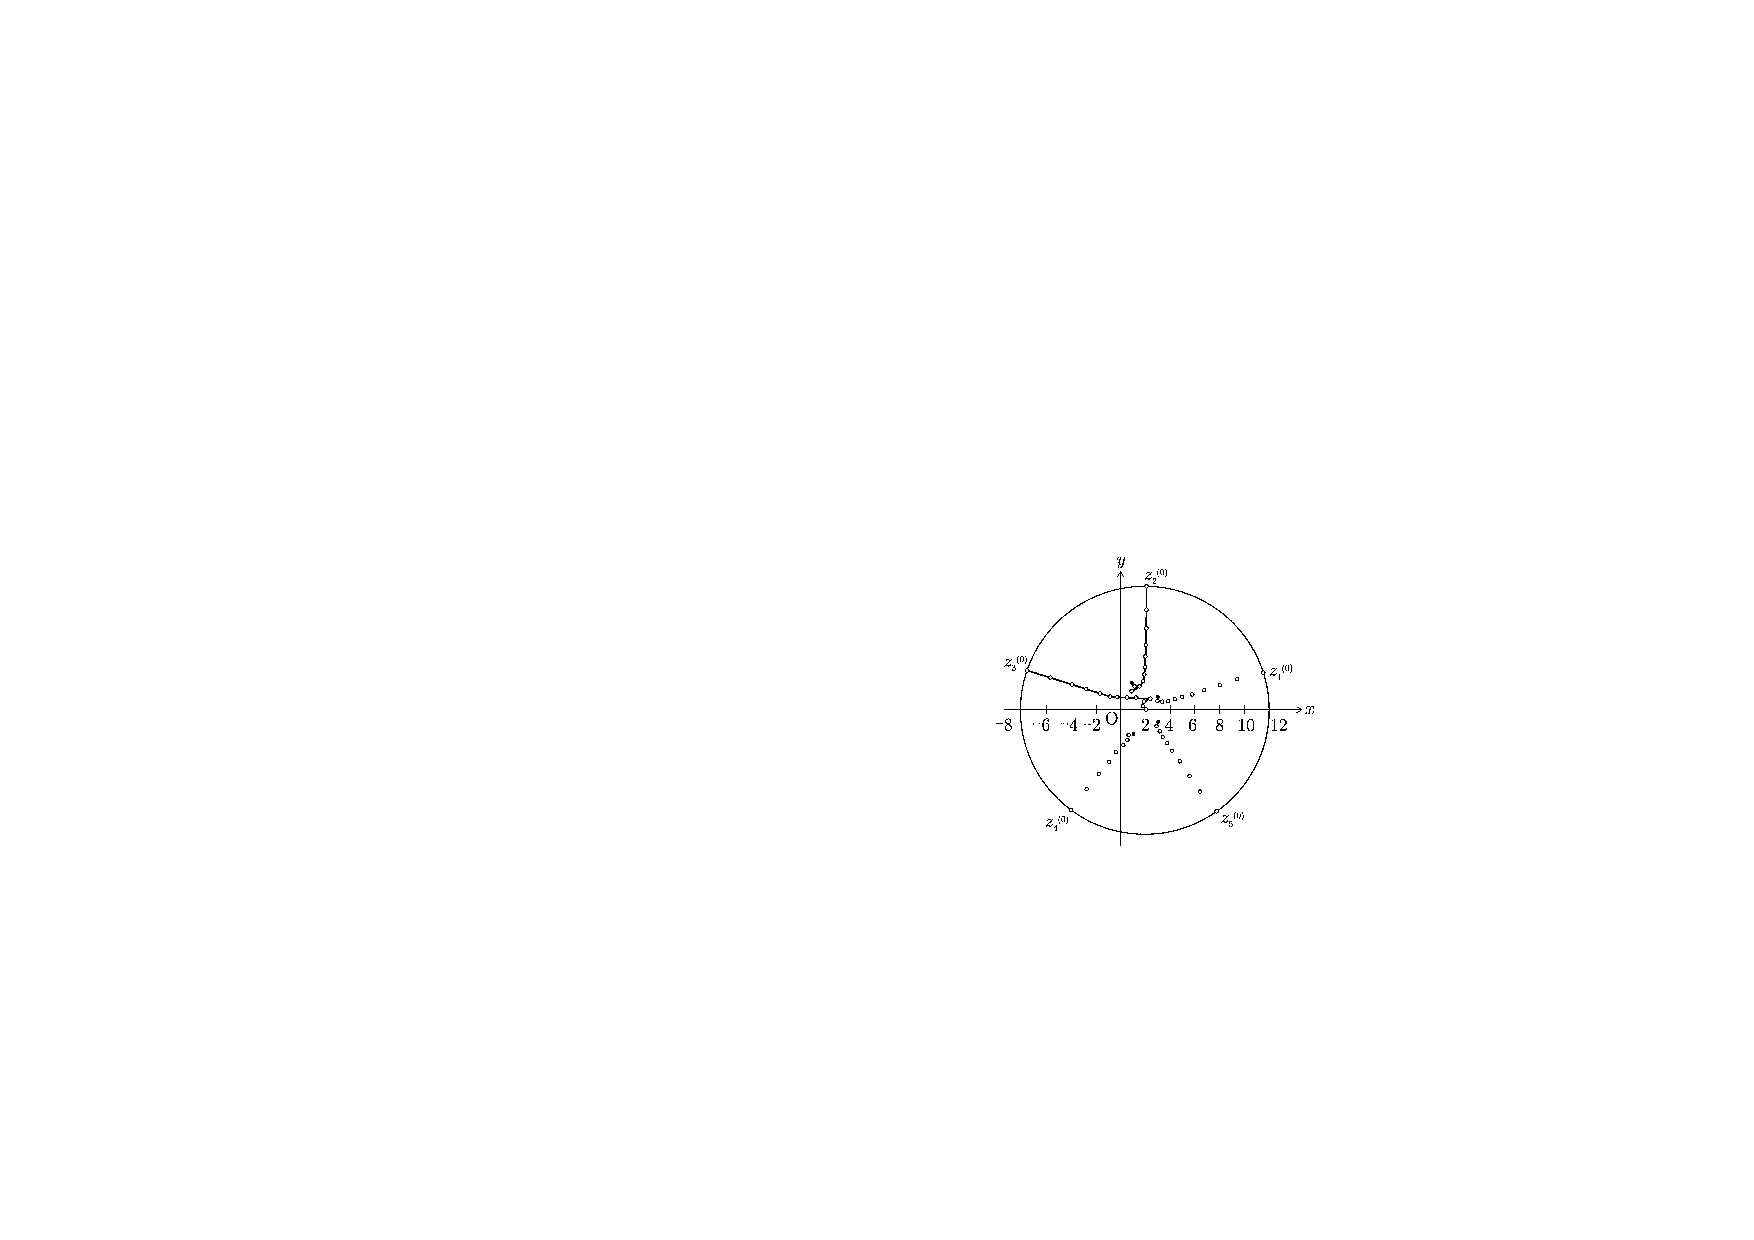
\includegraphics{image/DKA.pdf}}
\end{frame}

\section{C言語における行列の取り扱い}

\begin{frame}[t,fragile]{一次元配列}
  \begin{itemize}
    \setlength{\itemsep}{1em}
  \item (静的)一次元配列 (ハンドブック3.3.1節)
\begin{lstlisting}
double v[10];
v[0] = 1.0;
v[1] = 2.0;
...
\end{lstlisting}
    要素数はコンパイル時にすでに決まっている定数でなければならない
  \item (動的)一次元配列 (ハンドブック3.11節)
\begin{lstlisting}
double *v; /* ポインタ */
v = (double*)malloc((size_t)(10 * sizeof(double));
...
free(v); /* 確保した領域を開放 */
\end{lstlisting}
実行時に要素数を指定可能
  \end{itemize}
\end{frame}

\begin{frame}[t,fragile]{ポインタと一次元配列}
  \begin{itemize}
    \setlength{\itemsep}{1em}
  \item 一次元配列を表す変数は、(実は)最初の要素を指すポインタ  (ハンドブック3.5.3節)
    \begin{itemize}
    \item \verb+v+ と \verb+&v[0]+ は等価
    \item \verb^(v+2)^ と \verb^&v[2]^ は等価
    \item \verb+*v+ と \verb+v[0]+ は等価
    \item \verb^*(v+2)^ と \verb^v[2]^ は等価
    \item \verb^(v+2)[3]^ は?
    \end{itemize}
  \item C言語では配列の添字は0から始まることに注意
  \item \verb^double v[10];^ と宣言した場合、\verb^v[0]^ 〜 \verb^v[9]^ の10個の要素を持つ配列が作られる。\verb^v[10]^ は存在しない。値を代入したり参照しようとするとエラーとなる
  \end{itemize}
\end{frame}

\begin{frame}[t,fragile]{二次元配列}
  \begin{itemize}
    \setlength{\itemsep}{1em}
  \item C言語では、二次元配列は一次元配列の先頭をさす(ポインタ)の配列として表される(と理解しておけば良い)
  \item \verb+m[i]+は、要素\verb+m[i][0]+を指すポインタ
    \begin{itemize}
    \item \verb+m+ と \verb+&m[0]+ は等価 (\verb+&m[0][0]+ ではない)
    \item \verb+m[0]+ と \verb+&m[0][0]+ は等価
    \item \verb+m[2]+ と \verb+&m[2][0]+ は等価
    \item \verb^(m+2)^ と \verb^&m[2]^ は等価
    \item \verb^(*(m+2))[3]^ と \verb^*(*(m+2)+3)^ と \verb^m[2][3]^ は等価
    \item \verb^*(m+2)[3]^ と \verb^*((m+2)[3])^ と \verb^*(m[5])^ と\verb^m[5][0]^ は等価
    \item \verb^[]^は\verb^*^よりも強い
    \end{itemize}
  \end{itemize}
\end{frame}

\begin{frame}[t,fragile]{動的二次元配列の確保}
  \begin{itemize}
    \setlength{\itemsep}{1em}
  \item 各行を表す配列とそれぞれの先頭アドレスを保持する配列の二種類が必要
\begin{lstlisting}
double **a;
m = 10;  
n = 10;  
a = (double**)malloc((size_t)(m * sizeof(double*));
for (int i = 0; i < m; ++i)
  a[i] = (double*)malloc((size_t)(n * sizeof(double));
\end{lstlisting}
\item 各行を保持する配列が、メモリ上で連続に確保される保証はない
\item LAPACKを使うときに問題となる
  \end{itemize}
\end{frame}

\begin{frame}[t,fragile]{動的二次元配列の確保}
  \begin{itemize}
    \setlength{\itemsep}{1em}
  \item 二次元配列の要素を格納する長い配列を用意する
\begin{lstlisting}
double **a;
m = 10;  
n = 10;  
a = (double**)malloc((size_t)(m * sizeof(double*));
a[0] = (double*)malloc((size_t)(m*n * sizeof(double));
for (int i = 1; i < m; ++i)
  a[i] = a[i-1] + n;
\end{lstlisting}
  \item 開放は逆の順序で行う
\begin{lstlisting}
free(a[0]);
free(a);
\end{lstlisting}
  \end{itemize}
\end{frame}

\begin{frame}[t,fragile]{動的二次元配列の確保}
  \begin{itemize}
    \setlength{\itemsep}{1em}
  \item 二次元配列の確保({\tt alloc\_dmatrix})、開放({\tt free\_dmatrix})、出力({\tt print\_dmatrix})、読み込み({\tt read\_dmatrix})を行うためのユーティリティ関数を準備
  \item 実習用ワークステーションの{\tt /home/public/ce2015/ex3/matrix\_util.h}に置いてある
  \item 使用例
\begin{lstlisting}
#include "matrix_util.h"
...
double **mat;
mat = alloc_dmatrix(m, n);
...
free_dmatrix(mat);
\end{lstlisting}
  \end{itemize}
\end{frame}

\section{LAPACKライブラリ}

\begin{frame}[t,fragile]{LAPACK (Linear Algebra PACKage)}
  \begin{itemize}
    \setlength{\itemsep}{1em}
  \item 線形計算のための高品質な数値計算ライブラリ
    \begin{itemize}
    \item \url{http://www.netlib.org/lapack}
    \item 線形方程式、固有値問題、特異値問題、線形最小二乗問題など
    \item (FFT 高速フーリエ変換は入っていない)
    \item LAPACK自体はFortranで書かれている
    \end{itemize}
  \item ほぼ全てのPC、ワークステーション、スーパーコンピュータで利用可 (インストール済)
  \item Netlibでソースが公開されているリファレンス実装は遅いが、それぞれのベンダー(Intel、Fujitsu、etc)による最適化されたLAPACKが用意されている場合が多い(MKL、SSL2、etc)
  \item LAPACKを使うことにより、高速で信頼性が高く、ポータブルなコードを書くことが可能になる
  \end{itemize}
\end{frame}

\begin{frame}[t,fragile]{LAPACKによる連立一次方程式の求解}
  \begin{itemize}
    \setlength{\itemsep}{1em}
  \item LU分解を行うサブルーチン {\tt dgetrf} \\
    \url{http://www.netlib.org/lapack/explore-html/d3/d6a/dgetrf_8f.html}
  \item Fortranによる関数宣言
\begin{lstlisting}
subroutine dgetrf(integer M, integer N,
         double precision, dimension(lda, *) A,
         integer LDA, integer, dimension(*) IPIV,
         integer INFO)
\end{lstlisting}
\item {\tt A}: 左辺の行列、{\tt N,M}: 次元、{\tt IPIV}: 選択されたピボット行のリスト、{\tt lda}: {\tt M}と同じで良い
  \end{itemize}
\end{frame}

\begin{frame}[t,fragile]{LAPACKによる連立一次方程式の求解}
  \begin{itemize}
    \setlength{\itemsep}{1em}
  \item C言語から呼び出すための関数宣言を作成 (ハンドブック3.6.4節)
\begin{lstlisting}
void dgetrf_(int *M, int *N, double *A,
             int *LDA, int*IPIV, int *INFO);
\end{lstlisting}
関数名は全て小文字。関数名の最後に {\tt \_} (下線)を付ける
\item LU分解の例
\begin{lstlisting}
M = 10;
N = 10;
LDA = 10;
dgetrf_(&M, &N, &A[0][0], &LDA, &IPIV[0], &INFO);
\end{lstlisting}
完全なソースコードは、実習用ワークステーションの{\tt /home/public/ce2015/ex3/lu\_decomp.c}に置いてある
  \end{itemize}
\end{frame}

\begin{frame}[t,fragile]{CからFortranのライブラリを呼び出す際の注意事項}
  \begin{itemize}
    \setlength{\itemsep}{1em}
  \item スカラーも配列も全てポインタ渡しとする
  \item C言語は添字が0から始まる。Fortranは1から始まる
  \item CとFortranで、二次元配列のメモリ上での並びが違う \\
    Cはrow-major: {\tt a[0][0], a[0][1], a[0][2], $\cdots$} \\
    Fortranはcolumn-major: {\tt a(1,1), a(2,1), a(3,1), $\cdots$} \\
  \item Cで作成した行列をFortranに渡すと転置されてしまう
  \item コンパイル時には{\tt -llapack}オプションを指定し、LAPACKライブラリをリンクする(ハンドブック3.1.6節)
  \end{itemize}
\end{frame}

\end{document}
